\section{Hypothesis 1}

Hypothesis 1 (H1) is stated as follows:

\begin{quote}
Explore some of the hyperparameters available during the feature extraction
process. The hypothesis is that using hyperparameter values more suited to
birdsong classification problems will yield a higher classification accuracy.
\end{quote}

H1 was applied to two feature extraction processes that appear in some form
widely in the literature related to birdsong classification: MFCC and GTCC\@.

\subsection{MFCC}

The key argument under test in this work as mentioned in
Section~\ref{sssec:mfcc} is the \texttt{BandEdges} argument. The results for the
AUC and classification accuracy for the 7 experiments listed in
Table~\ref{table:h1_mfcc_experiments} for MFCC can be seen in
Table~\ref{table:hyp1_mfcc} and can be visualized in Figure~\ref{fig:hyp1_mfcc}.

\begin{table}[h!t]
\begin{center}
\begin{tabular}{cc c|c c}
\toprule
& \multicolumn{2}{c|}{AUC} & \multicolumn{2}{c}{Accuracy} \\
  Experiment & Linear & RBF & Linear & RBF \\ [0.5ex]
\midrule
  1 & \cellcolor{lightgray} 0.887 & \cellcolor{lightgray} 0.958 & 0.825 & 0.872 \\
  2 & 0.879 & 0.830 & \cellcolor{lightgray} 0.828 & 0.801 \\
  3 & 0.868 & 0.860 & 0.802 & 0.789 \\
  4 & 0.845 & 0.836 & 0.765 & 0.785 \\
  5 & 0.873 & 0.953 & 0.813 & \cellcolor{lightgray} 0.880 \\
  6 & 0.863 & 0.929 & 0.809 & 0.878 \\
  7 & 0.879 & 0.905 & 0.827 & 0.823 \\
\bottomrule
\end{tabular}
\caption{The AUC and classification accuracy scores for linear and RBF models
for different experiments for MFCC\@. The highest evaluation scores for each metric
and for each model are highlighted in grey.}\label{table:hyp1_mfcc}
\end{center}
\end{table}

\begin{figure}[ht]
  \centering
  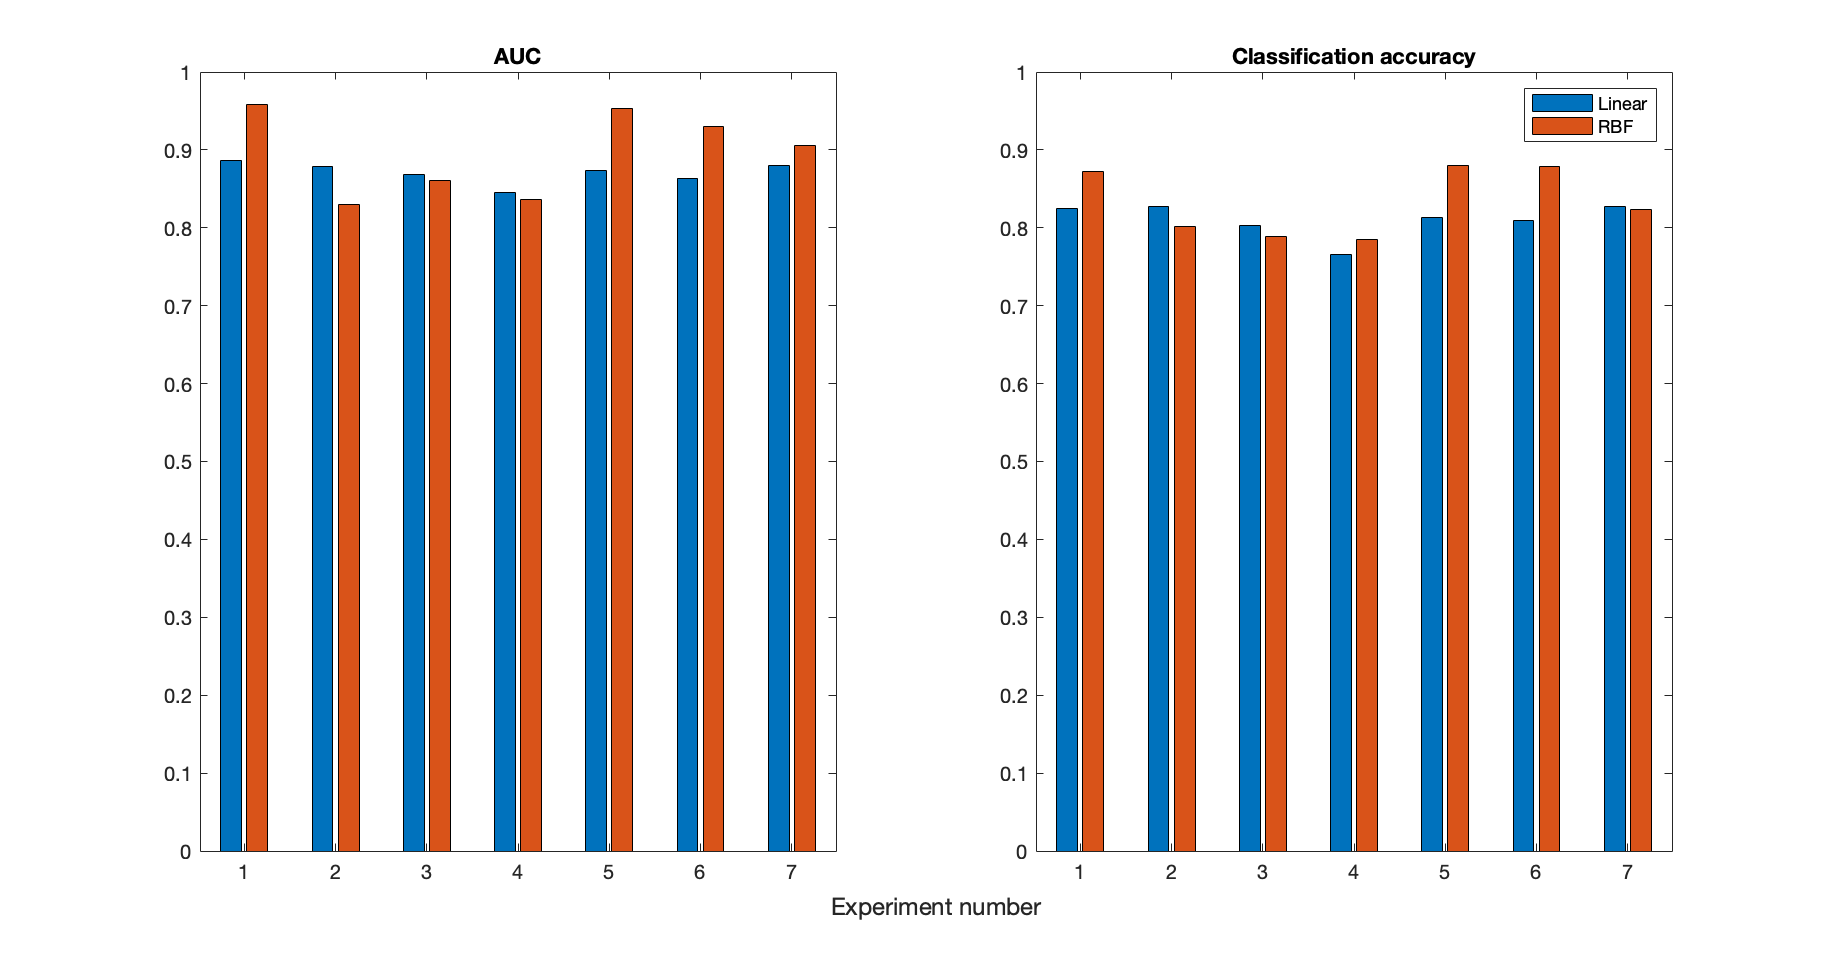
\includegraphics[width=\textwidth]{figures/hyp1_mfcc.png}
  \caption{The AUC and classification accuracy scores for linear and RBF models
  for different experiments for MFCC.}\label{fig:hyp1_mfcc}
\end{figure}

As shown in the table and chart, both evaluation metrics are around their
maximum in the control experiment (Experiment 1). Experiment 5 returns
comparable metrics to the control experiment, with slight improvements made to
the classification accuracy for the RBF model, but a slight reduction in the
AUC\@. The RBF model shows a clear reduction in performance for wider frequency
ranges across both evaluation metrics.

\subsection{GTCC}

The key argument under test in this work as mentioned in
Section~\ref{sssec:gtcc} is the \\ \texttt{FrequencyRange} argument. The results
for the AUC and classification accuracy for GTCC can be seen in
Table~\ref{table:hyp1_gtcc} and can be visualized in Figure~\ref{fig:hyp1_gtcc}.

\begin{table}[h!t]
\begin{center}
\begin{tabular}{cc c|c c}
\toprule
& \multicolumn{2}{c|}{AUC} & \multicolumn{2}{c}{Accuracy} \\
  Experiment & Linear & RBF & Linear & RBF \\ [0.5ex]
\midrule
  1 & 0.884 & 0.895 & 0.844 & 0.802 \\
  2 & 0.887 & 0.946 & 0.831 & 0.856 \\
  3 & \cellcolor{lightgray} 0.891 & 0.933 & \cellcolor{lightgray} 0.852 & 0.850 \\
  4 & 0.883 & \cellcolor{lightgray} 0.948 & 0.846 & \cellcolor{lightgray} 0.859 \\
\bottomrule
\end{tabular}
\caption{The AUC and classification accuracy scores for linear and RBF models
for different experiments for GTCC\@. The highest evaluation scores for each metric
and for each model are highlighted in grey.}\label{table:hyp1_gtcc}
\end{center}
\end{table}

\begin{figure}[ht]
  \centering
  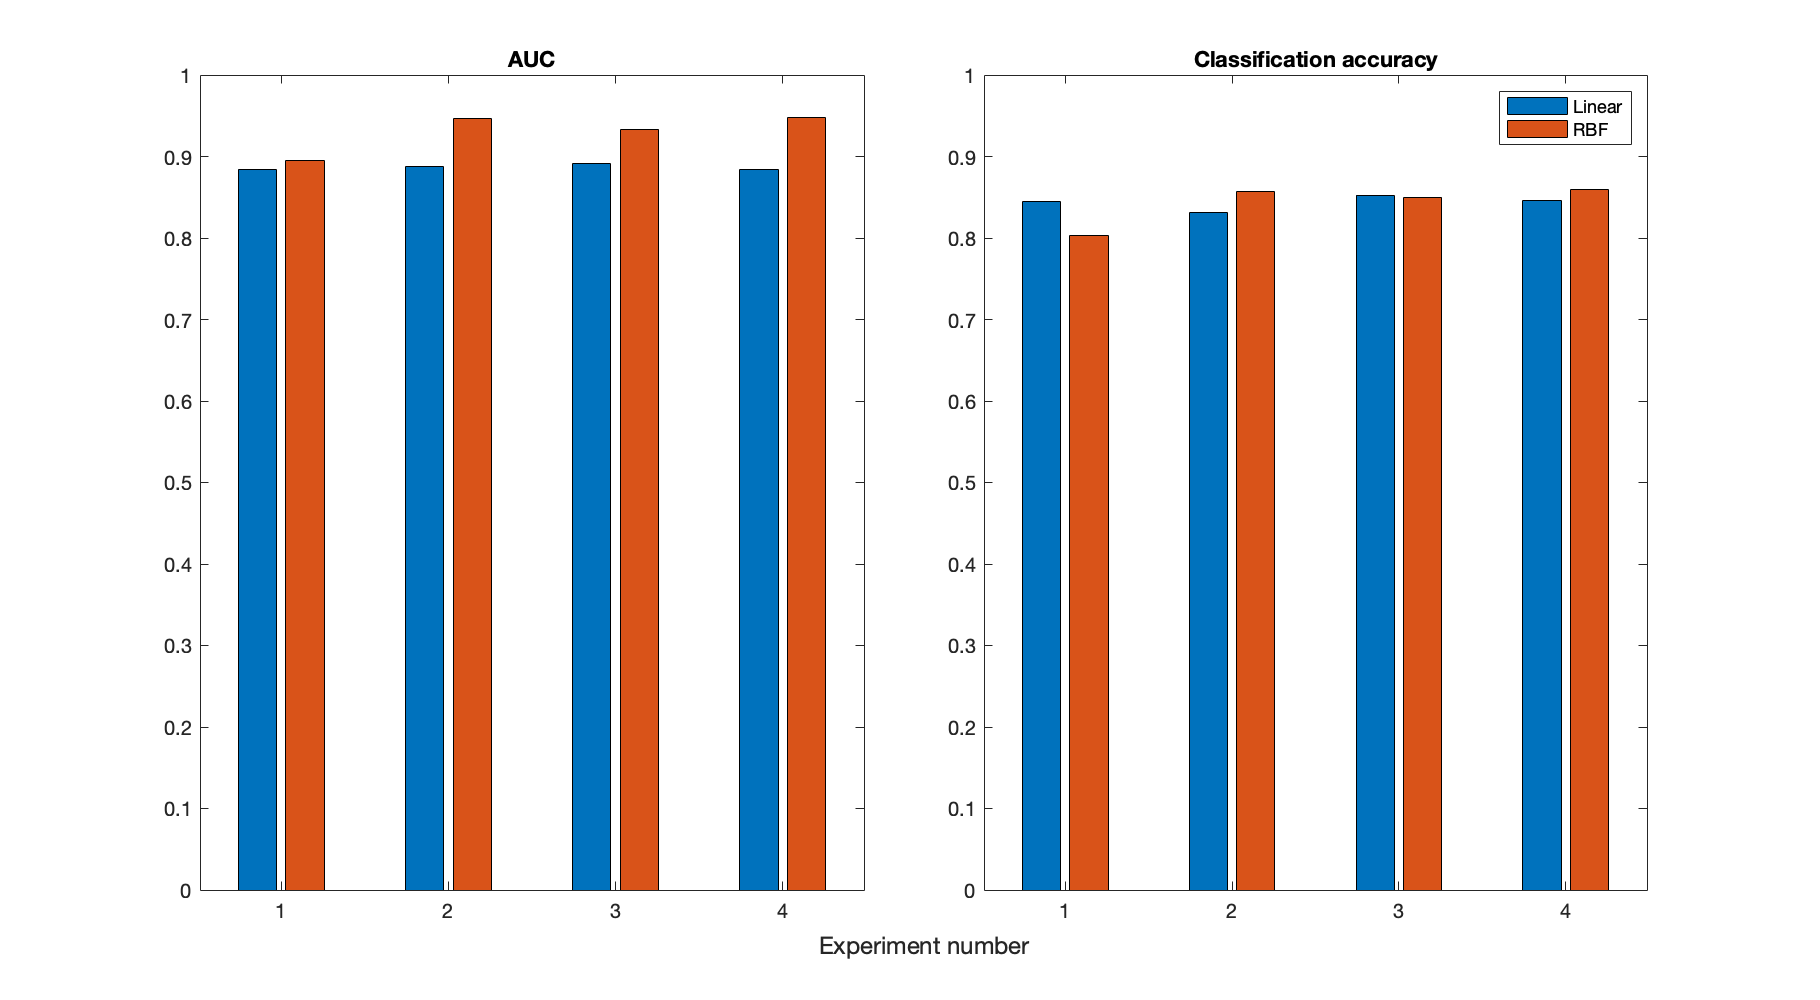
\includegraphics[width=\textwidth]{figures/hyp1_gtcc.png}
  \caption{The AUC and classification accuracy scores for linear and RBF models
  for different experiments for GTCC.}\label{fig:hyp1_gtcc}
\end{figure}

As shown in the table and chart, there is a significant increase in both metrics
for the RBF model when the frequency range is narrowed to be closer to the human
and birdsong vocalization range. The evaluation metrics for the linear model
remains largely similar across different frequency ranges.

\section{Hypothesis 2}

Hypothesis 2 (H2) is stated as follows:

\begin{quote}
Explore the performance of deep learning architectures such as Recurrent Neural
Networks (RNN) and Convolutional Neural Networks (CNN) and compare the results
with simpler statistical models. The hypothesis is that more complex and
flexible architectures such as these will have superior performance when
compared to simpler statistical models, such as SVMs.
\end{quote}

For all experiments related to H2 we use the highest performing feature
representation from H1: an MFCC representation with the \texttt{BandEdges}
argument set to the range from Experiment 1.

\subsection{CNN}

The CNN architectures listed in Table~\ref{table:cnn_architectures} will
be tested and their performance evaluated against the baseline: the highest
performing models from H1.

\subsubsection{Results}

The results for the AUC and classification accuracy for a CNN trained on a MFCC
representation of training sequences can be seen in
Table~\ref{table:cnn_mfcc_results} and can be visualized in
Figure~\ref{fig:cnn_mfcc_results}.

\begin{table}[h!t]
\begin{center}
\begin{tabular}{c c c}
\toprule
Model & AUC & Accuracy \\ [0.5ex]
\midrule
0 & 0.976 & 0.912 \\
1 & 0.971 & 0.865 \\
2 & \cellcolor{lightgray} 0.988 & \cellcolor{lightgray} 0.929 \\
\bottomrule
\end{tabular}
\caption{The AUC and classification accuracy for different CNN architectures
trained on MFCC feature representations. The highest evaluation scores for each
metric and are highlighted in grey.}\label{table:cnn_mfcc_results}
\end{center}
\end{table}

\begin{figure}[ht]
  \centering
  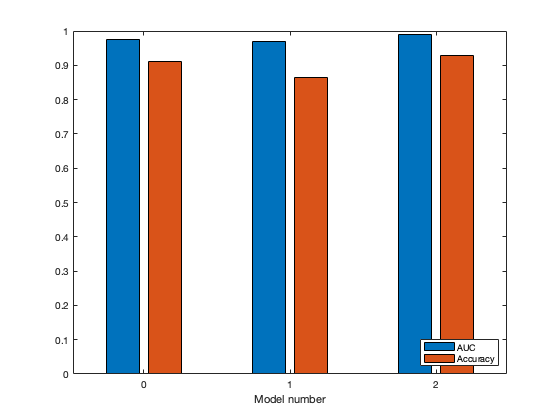
\includegraphics[width=0.8\textwidth]{figures/hyp2_cnn_mfcc_results.png}
  \caption{The AUC and classification accuracy for different CNN architectures
  trained on MFCC feature representations}\label{fig:cnn_mfcc_results}
\end{figure}

As can be seen, even the simplest CNN model (model 0) significantly outperforms
the most accurate SVM model in both AUC and accuracy. The highest performing of
the CNN models is model 3, but it should be noted that it takes significantly
longer to train model 3 compared to model 0 and its evaluation metrics are only
slightly better.

\section{Hypothesis 3}

Hypothesis 3 (H3) is stated as follows:

\begin{quote}
Explore the birdsong classification performance of feature representations
shown to have promising results for non-birdsong related audio classification
problems. The hypothesis is that feature representations shown to have good
results in audio classification problems will have good results for birdsong
identification.
\end{quote}

H3 was applied to a relatively novel feature representation, the MRCG, using
CNN\@. To the author's knowledge, this experiment has not been performed before
with regards to birdsong classification.

\section{Comparison}

\section{Discussion}
